13. Произведём 8 фиксированных переливаний, не зависящих от объёма второго кувшина. В конце этих действий если он окажется пустым, то он был 5-литровым, а в противном случае --- 6-литровым.
\begin{center}
\begin{figure}[h!]
\center{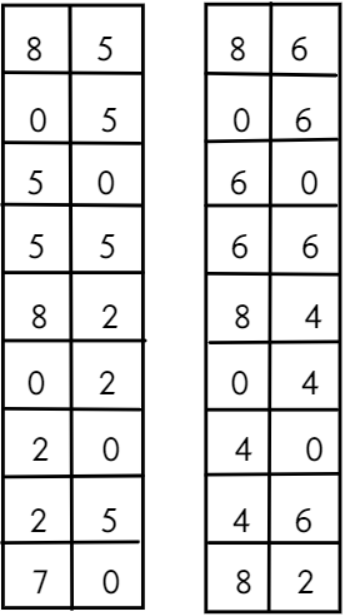
\includegraphics[scale=0.35]{s.png}}
\end{figure}
\end{center}

ewpage

oindent14. Произведём 8 фиксированных переливаний, не зависящих от объёма второго кувшина. В конце этих действий если он окажется пустым, то он был 3-литровым, а в противном случае --- 4-литровым.
\begin{center}
\begin{figure}[h!]
\center{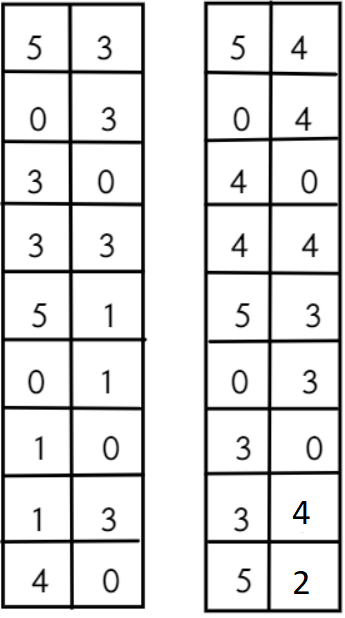
\includegraphics[scale=0.35]{ss.png}}
\end{figure}
\end{center}
